\chapter{热力学第一定律}\label{ch:b1:first-law}

给自行车打气，打气筒的筒身会热得握不住。
柴油机没有火花塞：它把空气压缩到原来的二十分之一，
空气热到足以自行点燃燃料。
压缩气体钢瓶在放空时，外壁会结霜。在每种情形中，
能量都在改变形式——功变成热，热变成功，两者又都
变成\omterm{def:b1:kinetic-theory:U}{内能}——而热力学第一定律正是使账目平衡的
记账规则。本章为\omterm{def:b1:first-law:transformation}{热力学系统}定义功
与热，陈述第一定律，引入作为其守恒量的
\omterm{def:b1:kinetic-theory:U}{内能}与焓，并将其应用于
\omterm{def:b1:kinetic-theory:model}{理想气体}的各种\omterm{def:b1:first-law:transformation}{过程}以及\omterm{met:b1:first-law:calorimetry}{量热学}。

\begin{omfigure}
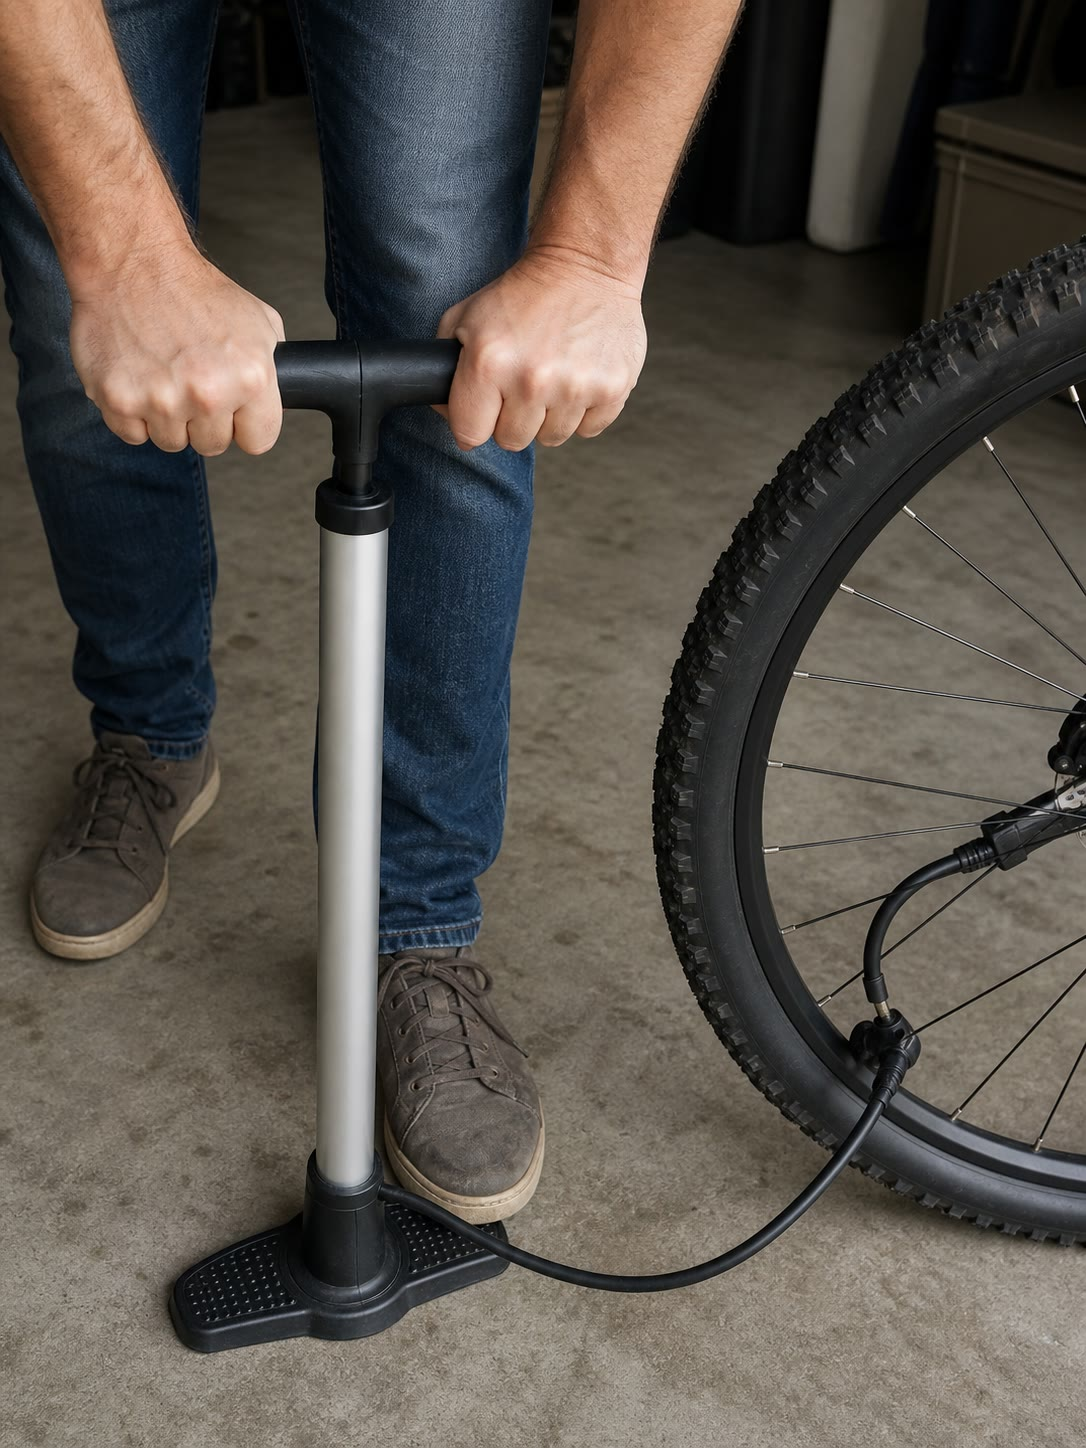
\includegraphics[width=0.36\linewidth]{images/book3/ai/b3-22-bicycle-pump.jpg}

{\small 自行车打气筒：手对被封闭空气所做的功使其\omterm{def:b1:kinetic-theory:U}{内能}升高，筒身随之变热——掌中的热力学第一定律。}
\end{omfigure}

\section{过程、功与热}

\begin{definition}[系统、过程]\label{def:b1:first-law:transformation}
\index{热力学系统}\index{过程}\index{准静态过程}\index{可逆过程}
\emph{热力学系统}是选定边界内的物质；
其余一切称为\emph{外界}。\emph{过程}使系统
从一个平衡态变到另一个平衡态。若
系统经历一系列平衡态（足够缓慢，
使 $P$、$T$ 处处有定义），则称过程为\emph{准静态的}；若
此外，将外部条件反向即可使路径反向（无
摩擦，与外界无有限的温差或压强差），则称其为\emph{可逆的}。
按保持不变的量命名：\emph{等温}（$T$）、\emph{等压}
（$P$）、\emph{等容}（$V$）；不交换热量时称为\emph{绝热}；
若外界压强（温度）恒定，无论系统内部如何变化，则称为\emph{外压恒定}（\emph{单\omterm{def:b1:first-law:heat}{热源}}）
过程。
\end{definition}

\begin{proposition}[压力的功]\label{prop:b1:first-law:work}
\index{功!压力的}
体积改变 $\dd V$、所受外界压强为
$P_{\mathrm{ext}}$ 的系统接收的功为
\[
\delta W = -P_{\mathrm{ext}}\,\dd V, \qquad
W = -\int_{V_1}^{V_2}P_{\mathrm{ext}}\,\dd V .
\]
对于\omterm{def:b1:first-law:transformation}{准静态过程}，$P_{\mathrm{ext}} = P$（系统自身的
压强），$W = -\int P\,\dd V$ 等于路径在
克拉珀龙图中所围面积的相反数：压缩时为正，膨胀时为负。
\end{proposition}

\begin{proof}
面积为 $S$ 的活塞受外界以力
$P_{\mathrm{ext}}S$ 推动，向外移动 $\dd x$：外界对系统做功
$-P_{\mathrm{ext}}S\,\dd x = -P_{\mathrm{ext}}\,\dd V$。任意
边界都可看作许多这样的活塞的组合。准静态时，活塞处于
平衡，$P_{\mathrm{ext}} = P$，二者之差趋于零。
\end{proof}

\begin{definition}[热]\label{def:b1:first-law:heat}
\index{热}\index{热源}
\emph{热}（热量）$Q$ 是以宏观功以外的方式传给系统的能量
——通过分子在器壁上的碰撞（传导）、
流体的循环流动（对流）、辐射。
\emph{热源}是一个大到无论交换多少热量其温度都不变的
物体。全书的符号约定：$W$ 与 $Q$ 均指系统
\emph{接收}的量，进入系统时为正。
\end{definition}

\section{第一定律}

\begin{theorem}[热力学第一定律]\label{thm:b1:first-law:firstlaw}
\index{热力学第一定律}\index{内能}
\omterm{def:b1:newton-dynamics:conservation}{封闭系统}具有一个状态函数，即其\emph{\omterm{def:b1:kinetic-theory:U}{内能}}
$U$（广延量），使得对任意\omterm{def:b1:first-law:transformation}{过程}
\[
\Delta U + \Delta E_{k} = W + Q ,
\]
其中 $E_k$ 为宏观\omterm{thm:b1:work-and-energy:ke}{动能}（静止系统为零）：
以功和热的形式接收的能量储存为\omterm{def:b1:kinetic-theory:U}{内能}。$W$
与 $Q$ 各自依赖于路径，二者之和则不然。
\end{theorem}
\admitted

\begin{remark}[它说的是什么]\label{rem:b1:first-law:meaning}
它就是能量守恒，只是承认热是能量的一种
传递（焦耳的桨轮实验：一份测定的功使水
升高的温度，总与一份等量测定的热相同）。“$U$ 是状态
函数”意味着 $\Delta U$ 由初态与终态决定——
因此循环有 $\Delta U = 0$ 与 $W + Q = 0$：输出
功的热机必须接收热量。$U$ 的微观内容见
\cref{def:b1:kinetic-theory:U}。
\end{remark}

\begin{definition}[焓；热容]\label{def:b1:first-law:enthalpy}
\index{焓}\index{定压热容}
\emph{焓} $H = U + PV$ 是适用于
等压\omterm{def:b1:first-law:transformation}{过程}的状态函数。\emph{\omterm{prop:b1:kinetic-theory:Ugas}{定容
热容}与定压热容}为
\[
C_V = \left(\frac{\partial U}{\partial T}\right)_V, \qquad
C_P = \left(\frac{\partial H}{\partial T}\right)_P ,
\]
单位为 \unit{J/K}；每\omterm{def:b1:kinetic-theory:scales}{摩尔}的为 $C_{V,m}$、$C_{P,m}$；每千克的为比
热容 $c_V$、$c_P$。
\end{definition}

\begin{proposition}[定容热与定压热]\label{prop:b1:first-law:qvqp}
对于静止且仅通过压力交换功的系统：
\begin{itemize}
  \item 等容\omterm{def:b1:first-law:transformation}{过程}：$W = 0$，$Q_V = \Delta U$；
  \item 在外界压强为 $P_0$ 的两个状态之间的外压恒定
        \omterm{def:b1:first-law:transformation}{过程}：$Q_P = \Delta H$。
\end{itemize}
\end{proposition}

\begin{proof}
等容\omterm{def:b1:first-law:transformation}{过程}：$\dd V = 0$。外压恒定\omterm{def:b1:first-law:transformation}{过程}：$W = -P_0(V_2 - V_1)$，故 $Q = \Delta U +
P_0\Delta V = \Delta(U + PV)$，因为 $P_1 = P_2 = P_0$。
\end{proof}

\begin{proposition}[理想气体：$U$、$H$ 与迈耶关系]\label{prop:b1:first-law:gas}
\index{迈耶关系}\index{绝热指数}\index{焦耳定律}
对\omterm{def:b1:kinetic-theory:model}{理想气体}，$U$ 与 $H$ 仅依赖于 $T$（焦耳定律）：
$\dd U = C_V\,\dd T$，$\dd H = C_P\,\dd T$，且
\[
C_{P,m} - C_{V,m} = R, \qquad \gamma = \frac{C_P}{C_V}, \qquad
C_{V,m} = \frac{R}{\gamma - 1}, \quad C_{P,m} = \frac{\gamma R}{\gamma - 1} ;
\]
\omterm{prop:b1:kinetic-theory:Ugas}{单原子气体} $\gamma = 5/3$，常温下\omterm{prop:b1:kinetic-theory:Ugas}{双原子气体}为 $7/5$。
对
\cref{prop:b1:kinetic-theory:condensed}中的\omterm{prop:b1:kinetic-theory:condensed}{凝聚相}模型，$C_P \approx C_V = C$，且
$\dd U \approx \dd H = C\,\dd T$。
\end{proposition}

\begin{proof}
$H = U + nRT$；对 $T$ 求导。
由\cref{prop:b1:kinetic-theory:Ugas}可知 $C_{V,m} = \tfrac32 R$ 或 $\tfrac52 R$。
\end{proof}

\section{理想气体的过程}

\begin{proposition}[四种典型过程]\label{prop:b1:first-law:transformations}
\index{等温过程}\index{绝热过程}\index{拉普拉斯定律}
对 $n$ \omterm{def:b1:kinetic-theory:scales}{摩尔}\omterm{def:b1:kinetic-theory:model}{理想气体}：
\begin{itemize}
  \item 等容\omterm{def:b1:first-law:transformation}{过程}：$W = 0$，$Q = \Delta U = nC_{V,m}\Delta T$；
  \item 等压\omterm{def:b1:first-law:transformation}{过程}（准静态）：$W = -P\Delta V = -nR\Delta T$，$Q = \Delta H =
        nC_{P,m}\Delta T$；
  \item 等温\omterm{def:b1:first-law:transformation}{可逆过程}：$\Delta U = 0$，$W = -Q = -nRT\ln(V_2/V_1) =
        nRT\ln(P_2/P_1)$；
  \item 绝热\omterm{def:b1:first-law:transformation}{可逆过程}：$Q = 0$，$W = \Delta U = nC_{V,m}(T_2 - T_1)$，
        且沿该路径有（\emph{拉普拉斯定律}）
        \[
        PV^\gamma = \text{常量}, \qquad TV^{\gamma - 1} = \text{常量}, \qquad
        T^\gamma P^{1 - \gamma} = \text{常量} .
        \]
\end{itemize}
\end{proposition}

\begin{proof}
等容与等压\omterm{def:b1:first-law:transformation}{过程}：见前述命题。\omterm{prop:b1:first-law:transformations}{等温过程}：$W =
-\int nRT\,\dd V/V$。\omterm{prop:b1:first-law:transformations}{绝热过程}：$\dd U = \delta W$，即 $nC_{V,m}\dd T =
-P\,\dd V = -nRT\,\dd V/V$，故 $\dd T/T = -(\gamma - 1)\dd V/V$（利用
$R/C_{V,m} = \gamma - 1$）；积分得 $TV^{\gamma - 1}$ 为常数，其余形式
由 $PV = nRT$ 得到。
\end{proof}

\begin{omfigure}
\begin{tikzpicture}
\begin{axis}[omaxis, axis x line=bottom, axis y line=left, width=8.4cm, height=5.8cm, xlabel={$V$}, ylabel={$P$},
    xlabel style={at={(axis description cs:0.5,-0.08)}, anchor=north},
    xmin=0, xmax=4.5, ymin=0, ymax=4.5, xtick={1,2,4}, xticklabels={$V_1$,$V_2$,$V_1'$}, ytick=\empty]
  \addplot[omDef, thick, domain=0.5:4.4, samples=100] {2.0/x};
  \addplot[omThm, thick, domain=0.62:4.4, samples=100] {2.0/(x^1.4)};
  \addplot[omDef, thick, dotted, domain=0.5:4.4, samples=100] {3.2/x};
  \fill[omExo!25] (axis cs:1,0) -- plot[domain=1:2, samples=40] (\x,{2.0/\x}) -- (axis cs:2,0) -- cycle;
  \fill[omDef] (axis cs:2,1.0) circle (1.5pt);
  \node[omDef, font=\footnotesize, below] at (axis cs:3.6,0.52) {等温线 $T_1$};
  \node[omThm, font=\footnotesize, below left] at (axis cs:1.0,2.0) {绝热线};
  \node[omDef, font=\footnotesize, above] at (axis cs:2.7,1.22) {等温线 $T_2 > T_1$};
  \node[omExo, font=\footnotesize] at (axis cs:1.5,0.45) {$\abs W$};
\end{axis}
\end{tikzpicture}\qquad
\begin{tikzpicture}[font=\small, x=1cm, y=1cm]
  \draw[thick] (0,0) -- (3.2,0) -- (3.2,2) -- (0,2);
  \fill[omDef!15] (0,0) rectangle (2.0,2);
  \draw[thick, fill=omExo!40] (2.0,0.05) rectangle (2.3,1.95);
  \draw[-Stealth, omThm, very thick] (3.6,1.0) -- (2.35,1.0) node[pos=0.0, right] {$P_{\mathrm{ext}}S$};
  \draw[-Stealth] (2.0,-0.4) -- (1.4,-0.4) node[left] {$\dd x$};
  \node at (1.0,1.0) {气体，$P$};
  \node[font=\footnotesize] at (1.6,-0.9) {$\delta W = -P_{\mathrm{ext}}\,\dd V$};
\end{tikzpicture}

{\small 左：在克拉珀龙图中，准静态压缩中气体所获得的功
等于路径下方的面积；从同一点出发，
绝热线比等温线更陡（$\gamma > 1$）：
无热量散失地压缩气体会使其升温，并沿更高的等温线上升。
右：外界对活塞所做的功。}
\end{omfigure}

\begin{example}[打气筒与柴油机]\label{ex:b1:first-law:diesel}
空气（$\gamma = 1.4$）从 \qty{1}{bar}、\qty{300}{K} 绝热压缩到
\qty{7}{bar}（自行车打气筒）：$T_2 = 300 \times 7^{0.286} = \qty{523}{K}$
——瞬时达到 \qty{250}{\degreeCelsius}，筒壁会感到这一温度。
柴油机压缩比为 $20$：$T_2 = 300 \times 20^{0.4} = \qty{994}{K}$，
$P_2 = 20^{1.4} = \qty{66}{bar}$——高于
燃料的自燃温度，因此发动机无需火花塞点火（周末问题要求计算
整个循环）。
\end{example}

\begin{remark}[不可逆过程]\label{rem:b1:first-law:irreversible}
\index{焦耳膨胀}\index{不可逆过程}
\omterm{def:b1:first-law:transformation}{过程}非准静态时，拉普拉斯定律与 $W =
-\int P\,\dd V$ 不再适用；只有 $W = -\int P_{\mathrm{ext}}\,\dd V$ 和
第一定律仍然成立。两个经典例子：气体向真空膨胀（
\omterm{rem:b1:first-law:irreversible}{焦耳膨胀}）不做功，器壁绝热时也不吸热——$\Delta U
= 0$，\omterm{def:b1:kinetic-theory:model}{理想气体}的温度保持不变；若气体被突然压缩，
外压跃变到 $P_2$，则气体接收功 $W = -P_2\Delta V$，
比达到同一压强时的可逆功更多，末态温度更高（见
\cref{exo:b1:first-law:11}）。
\end{remark}

\section{量热学}

\begin{method}[量热平衡]\label{met:b1:first-law:calorimetry}
\index{量热学}\index{潜热}
置于绝热容器内、在恒定（大气）压强下相互接触的物体，
之间只交换热量：总焓变
$\Delta H = \sum Q_P = 0$。对每个物体，无相变时 $\Delta H = mc\,\Delta T$
；若在其相变温度下发生状态变化，则 $\pm mL$，
其中 $L$ 为\emph{潜热}（单位质量的熔化焓或汽化焓
：水在 \qty{0}{\degreeCelsius} 时 $L_f = \qty{334}{kJ/kg}$，在 \qty{100}{\degreeCelsius} 时 $L_v =
\qty{2260}{kJ/kg}$）。列出平衡方程，解出
末温，并检验每个物体的假定相态
与之是否相符。
\end{method}

\begin{example}[冰入水中]\label{ex:b1:first-law:ice}
将 \qty{50}{g} 的 \qty{0}{\degreeCelsius} 冰放入 \qty{200}{g}、\qty{30}{\degreeCelsius} 的水中：
熔化冰需要 \qty{16.7}{kJ}；水降温至 \qty{0}{\degreeCelsius} 时可放出
\qty{25.1}{kJ} 的热量，因此冰全部熔化，
由 $0.250 \times 4180 \times (T_f - 0) = 25.1 - 16.7$ kJ 可得
$T_f = \qty{8}{\degreeCelsius}$。若冰为 \qty{100}{g}，
则需 \qty{33.4}{kJ}：只有部分冰熔化，$T_f = \qty{0}{\degreeCelsius}$
——检验这一点很重要。
\end{example}

\begin{omfigure}
\begin{tikzpicture}
\begin{axis}[omaxis, axis x line=bottom, axis y line=left, width=10cm, height=5.2cm, xlabel={加热量 (\unit{kJ/kg})}, ylabel={$T$ (\unit{\degreeCelsius})},
    xlabel style={at={(axis description cs:0.5,-0.1)}, anchor=north},
    xmin=0, xmax=3200, ymin=-30, ymax=130, xtick={334,752,3012}, xticklabels={$334$,$752$,$3012$}, ytick={0,100}]
  \addplot[omDef, thick] coordinates {(0,-20) (42,0) (376,0) (794,100) (3054,100) (3154,120)};
  \node[omDef, font=\footnotesize, below] at (axis cs:200,-2) {熔化};
  \node[omDef, font=\footnotesize, above] at (axis cs:1900,102) {沸腾};
  \node[font=\footnotesize, right] at (axis cs:900,50) {液态水，$c = \qty{4.18}{kJ/(kg.K)}$};
\end{axis}
\end{tikzpicture}

{\small 将一千克 \qty{-20}{\degreeCelsius} 的冰加热至
水蒸气：每次相变期间温度保持不变，同时供给
潜热——熔化需 \qty{334}{kJ}，沸腾需 \qty{2260}{kJ}，
远多于使液体从 \qty{0}{} 升至
\qty{100}{\degreeCelsius} 所需的 \qty{418}{kJ}。}
\end{omfigure}

\section{练习}

\begin{exercise}[$\star$]\label{exo:b1:first-law:1}
将 1 \omterm{def:b1:kinetic-theory:scales}{摩尔}空气（$C_{P,m} = \qty{29.1}{J/(mol.K)}$）在恒定压强下由
\qty{300}{K} 加热至 \qty{400}{K}。
求吸收的热量、外界对其所做的功及\omterm{def:b1:kinetic-theory:U}{内能}变化。
\end{exercise}

\begin{exercise}[$\star$]\label{exo:b1:first-law:2}
1 \omterm{def:b1:kinetic-theory:scales}{摩尔}、\qty{300}{K} 的气体经等温
可逆压缩，体积由 \qty{2.0}{L} 变为 \qty{0.50}{L}。求外界做的功、
交换的热量及 $\Delta U$。
\end{exercise}

\begin{exercise}[$\star$]\label{exo:b1:first-law:3}
空气（\qty{300}{K}、\qty{1}{bar}）经绝热
可逆压缩，体积变为原来的十分之一。求末温与末压强。
\end{exercise}

\begin{exercise}[$\star$]\label{exo:b1:first-law:4}
求氩气和氮气的 $C_{V,m}$、$C_{P,m}$ 及 $\gamma$。对于
液态水（$c = \qty{4180}{J/(kg.K)}$），为何可以略去
$c_P$ 与 $c_V$ 的区别？
\end{exercise}

\begin{exercise}[$\star\star$]\label{exo:b1:first-law:5}
将 \qty{200}{g}、\qty{80}{\degreeCelsius} 的水与 \qty{300}{g}
、\qty{20}{\degreeCelsius} 的水在绝热杯中混合。求末温；若
杯子本身的热容为 \qty{80}{J/K}，
初温为 \qty{20}{\degreeCelsius}，结果有何变化？
\end{exercise}

\begin{exercise}[$\star\star$]\label{exo:b1:first-law:6}
将 \qty{50}{g}、\qty{-10}{\degreeCelsius} 的冰（$c_{\text{冰}} = \qty{2100}{J/(kg.K)}$）
投入 \qty{200}{g}、\qty{30}{\degreeCelsius} 的水中。求末态
与末温。若冰为 \qty{150}{g}，结果如何？
\end{exercise}

\begin{exercise}[$\star\star$]\label{exo:b1:first-law:7}
某气体沿克拉珀龙图上的矩形循环变化：$(V_1, P_1)
\to (V_2, P_1) \to (V_2, P_2) \to (V_1, P_2) \to (V_1, P_1)$，其中 $V_2 > V_1$，
$P_2 > P_1$。求一个循环中外界做的功，并将其表示为面积的函数；
给出其符号，并说明符号的含义。
\end{exercise}

\begin{exercise}[$\star\star$]\label{exo:b1:first-law:8}
自行车打气筒将 \qty{1}{bar}、\qty{300}{K} 的空气
迅速压缩至 \qty{7}{bar}，\omterm{def:b1:first-law:transformation}{过程}可视为绝热。求达到的温度；说明
打气筒为何会发热，以及
停止打气后轮胎气压为何会略有下降。
\end{exercise}

\begin{exercise}[$\star\star$]\label{exo:b1:first-law:9}
\omterm{def:b1:kinetic-theory:model}{理想气体}向一个真空的绝热容器中膨胀（\omterm{rem:b1:first-law:irreversible}{焦耳
膨胀}）。求功、热量、$\Delta U$、$\Delta T$。该\omterm{def:b1:first-law:transformation}{过程}是否可逆？
真实气体又会如何？
\end{exercise}

\begin{exercise}[$\star\star\star$]\label{exo:b1:first-law:10}
在 \qty{100}{\degreeCelsius}、\qty{1}{atm} 下将 \qty{1.0}{kg} 水煮沸
（水蒸气体积为 \qty{1.67}{m^3}）。求吸收的热量、与
大气交换的功及 $\Delta U$。大部分潜热去了哪里？
\end{exercise}

\begin{exercise}[$\star\star\star$]\label{exo:b1:first-law:11}
1 \omterm{def:b1:kinetic-theory:scales}{摩尔}\omterm{prop:b1:kinetic-theory:Ugas}{双原子气体}在 \qty{300}{K}、\qty{1}{bar} 下，置于绝热
汽缸中，突然将外压设为
\qty{5}{bar} 并等待达到平衡而被压缩。求末温与末体积
（用第一定律及 $W = -P_{\mathrm{ext}}\Delta V$）；并与可逆
绝热压缩至 \qty{5}{bar} 进行比较。
\end{exercise}

\begin{exercise}[$\star\star\star$]\label{exo:b1:first-law:12}
声音是快速压缩\omterm{def:b1:first-law:transformation}{过程}，因而是绝热的：其速率为 $c = \sqrt{\gamma P/\rho}$
（等温值 $\sqrt{P/\rho}$ 是牛顿的错误）。计算
\qty{20}{\degreeCelsius} 空气中两者的值，并与实测
的 \qty{343}{m/s} 比较。证明 $c = \sqrt{\gamma RT/M}$，并与在
\cref{ch:b1:kinetic-theory}中的\omterm{def:b1:kinetic-theory:kinetictemp}{方均根速率}比较。
\end{exercise}

\section{问题：从自行车打气筒到柴油机}

\begin{problem}[{周末问题——一个让手指发烫的手动打气筒，
一个自己点燃燃料的气缸，以及在空气垫上弹跳的钢球：
三次压缩中的第一定律}]
\label{pb:b1:first-law:1}
空气：理想\omterm{prop:b1:kinetic-theory:Ugas}{双原子气体}，$\gamma = 1.40$，$C_{V,m} = \tfrac52 R$，$C_{P,m} =
\tfrac72 R$，$M = \qty{29}{g/mol}$；$R = \qty{8.314}{J/(mol.K)}$。各处的初始
状态为：$P_1 = \qty{1.00}{bar}$，$T_1 = \qty{300}{K}$。

\medskip
\noindent\textbf{第一部分——自行车打气筒。}
打气筒的气缸体积为 $V_1 = \qty{212}{cm^3}$；其中的空气
被可逆绝热压缩，直至压强达到轮胎的
压强 \qty{7.0}{bar}。
\begin{enumerate}
  \item 气缸中空气的量。
  \item 压缩结束时的体积。
  \item 压缩结束时的温度。
  \item 一次冲程中空气所接受的功。
  \item 轮胎（\qty{2.0}{L}）须在 \qty{300}{K} 下由 \qty{1}{bar} 充至
        \qty{7}{bar}：需要多少次冲程，总共需要多少功
        （每次冲程的功视为常量）？
  \item 热空气随后在轮胎内冷却至 \qty{300}{K}，
        轮胎压强会发生什么变化，骑车人该怎么做？
  \item 比较每次冲程的绝热功与将气体等温压缩至同一
        \qty{7}{bar} 的功。为何等温功更大，
        尽管此时气体的终温更低？
\end{enumerate}

\medskip
\noindent\textbf{第二部分——柴油机的压缩。}
一个体积为 $V_1 = \qty{0.50}{L}$ 的气缸将其中空气可逆绝热压缩，
体积压缩了 $20$ 倍。
\begin{enumerate}[resume]
  \item 压缩后空气的量，以及温度 $T_2$。
  \item 压强 $P_2$。
  \item 燃料在约 \qty{500}{K} 以上自燃：解释为何柴油机
        不需要火花塞，以及为何汽油机（压缩比
        $\approx 10$，见 \cref{exo:b1:first-law:3}）必须避免自燃。
  \item 压缩\omterm{def:b1:first-law:transformation}{过程}中空气所接受的功。
  \item 转速为 \qty{3000}{rpm} 时，一个气缸每秒压缩 $25$ 次：
        压缩所吸收的功率（该能量会在循环后段
        释放出来）。
  \item 实际的压缩\omterm{def:b1:first-law:transformation}{过程}很快（不可逆），并向器壁散热：
        每种效应使 $T_2$ 向哪个方向变化？
\end{enumerate}

\medskip
\noindent\textbf{第三部分——燃烧与膨胀。}
活塞到达冲程顶端时，\qty{20}{mg} 燃料（热值
\qty{43}{MJ/kg}）在活塞开始下行时，于定压
$P_2$ 下燃烧；随后气体可逆绝\omterm{prop:b1:kinetic-theory:condensed}{热膨胀}回到 $V_1$。
全程将气体视为空气。
\begin{enumerate}[resume]
  \item 燃料释放的热量。
  \item 燃烧结束时（定压\omterm{def:b1:first-law:transformation}{过程}）的温度 $T_3$ 与
        体积 $V_3$。
  \item 定压阶段交换的功（注意符号）。
  \item 绝\omterm{prop:b1:kinetic-theory:condensed}{热膨胀}结束时的温度 $T_4$，以及
        该\omterm{def:b1:first-law:transformation}{过程}中交换的功。
  \item 气体在四个冲程中输出的净功，以及
        它与放出热量之比（即理想效率）。
  \item 将该效率与 $1 - T_1/T_3$ 比较，后者是
        在\cref{ch:b1:heat-engines}中将为任一工作于这两个极端温度之间的热机
        所建立的界限。
  \item 由整个循环的第一定律求排气所放出的热量；
        并校验能量平衡。
\end{enumerate}

\medskip
\noindent\textbf{第四部分——用弹跳的钢球测量 $\gamma$。}
一个质量为 $m = \qty{16.5}{g}$ 的钢球放入竖直的玻璃管中，管的
横截面积为 $S = \qty{2.0}{cm^2}$，底部由一只装有空气的烧瓶封闭，
烧瓶的体积为 $V = \qty{10}{L}$，压强为 $P = \qty{1.0}{bar}$；
小球从平衡位置偏移 $x$ 后即做振动。
\begin{enumerate}[resume]
  \item 为何可以将空气的压缩与膨胀视为
        \omterm{prop:b1:first-law:transformations}{绝热过程}？写出小位移 $x$ 与压强变化
        $\dd P$ 之间的关系（拉普拉斯定律，线性化）。
  \item 求出作用于小球的回复力，并证明其运动
        为谐振动，且 $\omega_0^2 = \gamma PS^2/mV$。
  \item 计算周期，以及由测得的周期 \qty{1.10}{s}
        所推出的 $\gamma$ 值。
  \item 为何小球与管壁间的摩擦及空气泄漏会使结果
        产生偏差？偏差沿哪个方向？
  \item 总结三次压缩：第一定律在各次压缩中分别守恒的量，
        以及\omterm{prop:b1:first-law:gas}{绝热指数} $\gamma$
        所支配的量。
\end{enumerate}
\end{problem}
